\documentclass[runningheads]{llncs}

\usepackage{graphicx}
\usepackage{booktabs}

% Package for todo command
\usepackage{xcolor}

\newcommand\todo[1]{\textcolor{red}{#1}}

\begin{document}

\title{My Cool Title}

\author{Jacobus C. Lock\inst{1} \and
  Grzegorz Cielniak\inst{1} \and
  Andrea Tramontano\inst{2} \and
  Nicola Bellotto\inst{1}
}
\authorrunning{J.C. Lock et. al.}
\institute{University of Lincoln, Lincoln, UK \and
  Universita Degli Studi Di Padova, Italy
}

\maketitle

\begin{abstract}
  Cool abstract here
  \keywords{All the best keywords}
\end{abstract}

\section{Introduction}

It is estimated that there are almost half a billion people today that live with mild to severe levels of vision impairments or total blindness and this number is expected to significantly rise with an ageing population~\cite{bourne2017magnitude}.
There has been a rise interest from industrial partners in utilising modern technology to make their products more accessible and improvements in modern computing power and image processing capabilities have made this easier.
The work we present here is part of the ActiVis project that aims to assist people with vision impairments (PwVI) to independently navigate and find objects within an unknown indoor environment using only a mobile phone and its camera.
This system implements ideas from the active vision field~\cite{bajcsy2017,bellotto2013}, but replaces the electro-mechanical servo typically found in active vision systems, with a user's arm and hand as pictured in Fig.~\ref{fig:system-in-use}.
This project expands upon concepts originally proposed in~\cite{bellotto2013} and~\cite{lock2017portable} and builds off of the system introduced in~\cite{lock2019active}.

\begin{figure}
  \centering
  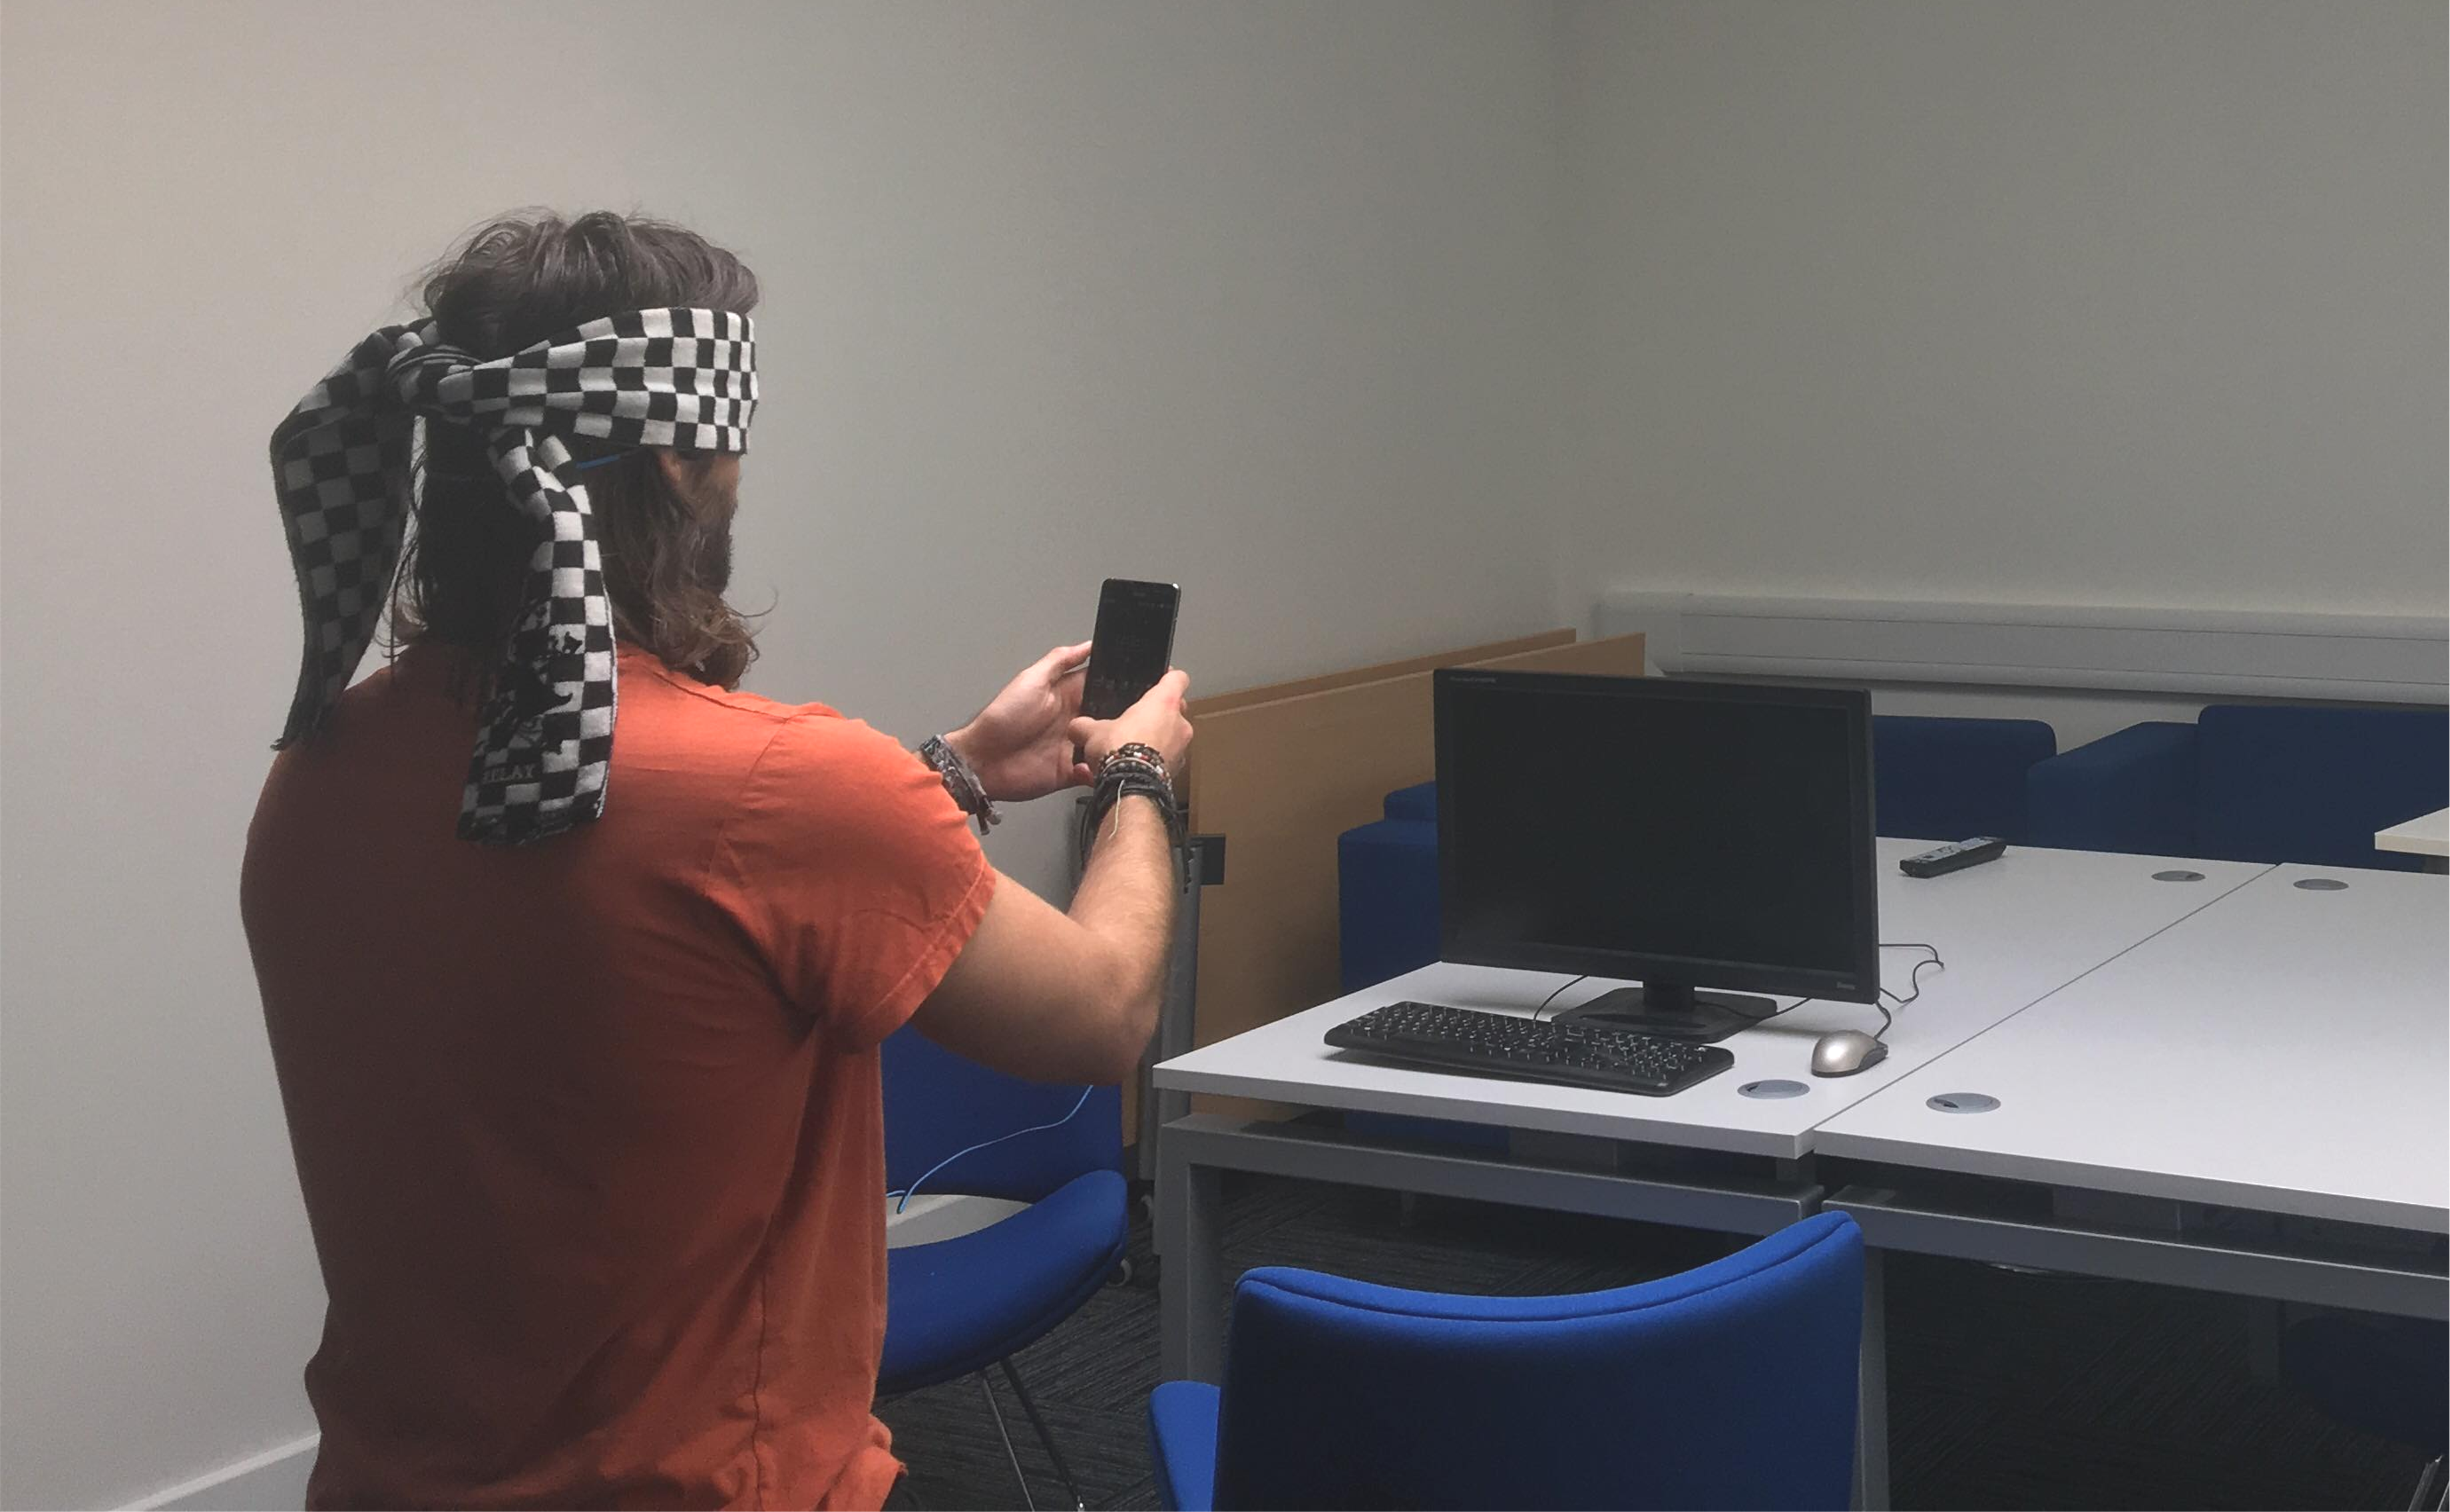
\includegraphics[width=0.5\textwidth]{figures/system_use.png}
  \caption{The system in use during an experiment. }\label{fig:system-in-use}
\end{figure}

Our active search system uses the camera's current and previous views as input and leverages its understanding of inter-object spatial relationships to determine the best navigation action to determine the best action to take to reach the target object.
To enable this, we expanded upon our previous work and implemented a partially observable Markov Decision Process (POMDP)~\cite{bellman1957markovian} on a mobile phone generates real-time navigation instructions to guide the user to their target object.

This work includes the following contributions:

\begin{itemize}
  \item a POMDP-based human controller that enables object search and guidance on a mobile phone;
  \item experiments that evaluate the efficacy of the proposed system.
\end{itemize}

\todo{Add paper layout}

\section{Previous Work}

\section{Active Vision System}

The work we present in this paper is an advancement towards the ActiVis projects larger goal of developing a stand-alone mobile system that can guide a PwVI towards their desired destination with minimal user input or intervention. 
This work focuses on guiding a user towards an object in one, static environment and is limited to 2 dimensions (pan and tilt).

A complete system diagram is given in Fig.~\ref{fig:sys-diagram}\todo{cite own work where fig is from if necessary}. 
This diagram shows a typical feedback control loop that generates a control signal to minimise some error signal, but has been modified to incorporate a human within the loop.

\begin{figure}
  \centering
  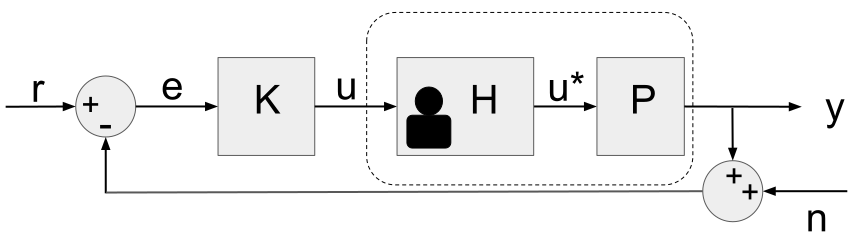
\includegraphics[width=0.75\textwidth]{figures/control_loop.png}
  \caption{System control loop: $r$ is the reference object, $e$ the error signal, $u$ and $u^*$ the original and interpreted control signals and $y$ is the current object observation. $K$, $H$ and $P$ are the control, human and sensor blocks respectively. }\label{fig:sys-diagram}
\end{figure}

In this case, the error is defined as the difference between the desired object and the object currently within view. 
The implication of this modification is that an additional block, \emph{H}, is added to simulate a human that receives an control signal, \emph{u}, from the controller, \emph{K}. 
However, the challenge with people is that a person may interpret \emph{u} in any unpredictable way (i.e.\ apply a transformation) that results in the signal \emph{u*} that points the camera, \emph{P}, to a new location containing a new object observation, \emph{y}.
It is therefore important to design \emph{K} to take be robust enough to accommodate different user habits and limitations and ensure that \emph{u*} tracks \emph{u} as closely as possible. 
These design considerations are addressed in previous work. \todo{how to state that we designed the interface already if its unpublished?}

Another fact to take note of is the measurement noise, \emph{n}, added in the feedback loop that simulates an object detector making classification errors that will influence the action that \emph{K} generates. 
In our previous work, we assumed a `perfect classifier' and solved the problem using a plain Markov decision process (MDP). 
In this work we do away with that somewhat naive assumption and implement a POMDP that can better handle the observation uncertainties inherent to modern object detectors and classifiers. 
The design of the human controller is discussed next. 

\section{Experiment Design}

To evaluate the effectiveness of our POMDP controller and guidance system, we designed a set of experiments that can measure its performance in driving a user towards a target object within the environment. 
We also conducted an additional set of experiments with an alternative guidance system to act as a baseline measurement to compare our results to and provide additional context. 
This alternative `guidance' system does not actually provide any guidance instructions to the user, instead it provides the user with the raw observation output from the object classifier and makes use of the user's intuition and prior environment knowledge to generate actions. 
The goal of both the guided and unguided experiment cases were to find an object within a static environment. 

We recruited 10 sighted participants that were blindfolded for the experiments, as well as 2 legally blind participants, where 1 was blind from birth and the other suffers from late onset blindness\todo{Give participant stats}.
Details on the design of these experiments are given in the next sections. 

\subsection{Unguided Case}

The design goal of this experiment is to mimic how a typical person with healthy eyesight would behave if told to look for a given object. 
In such a scenario, a person would exploit the objects currently within their view and their prior knowledge on a room's typical layout to make a decision on where to look next to find what they are looking for. 
Take for example a person in bathroom facing the basin after washing their hands and looking for a hand-dryer. 
It is unlikely that a hand dryer would be placed above or below a wash basin so it it is reasonable to believe that they would instinctively look at chest height on the walls to their left, right or behind them to find a dryer. 

For this experiment, a mobile camera and object detector acts as the participant's eyes and informs them what the objects within the camera's view and it is then up to the participant to exploit their prior knowledge of the given environment in order to manipulate the camera to point towards the target object. 
This process is modelled by the schematic in Fig. MEME\todo{put in figure without controller} where the human, \emph{H}, acts as both the actuator and controller.
The object detector was implemented in an Android app that uses the object classifier and Android's Text-to-Speech engine to read out any objects that it detected. 
The app only reads out the objects when the participant requested it to by tapping on the screen. 
When the target object comes within the camera's view and is correctly classified by the object detector, the device vibrated to inform the participant. 

Each participant was verbally told what the target object was they they were meant to find and each participant was given 45 seconds to find the target object. 
In this case, the learning effect was ignored in order to mimic the typical search behaviour described earlier. 
Each experiment run was ended when a target was found or the time limit was reached. 
This process was repeated a total of 8 times, once for each target object within the environment. 

\subsection{Guided Case}

In this experiment, we evaluate the performance of the guidance system in the object search task, where the perception and control tasks are performed by the guidance system and mobile device and the participant acts as the actuator, interpreting control signals and outputting actuation forces on the camera sensor. 
This is modelled by the schematic in Fig.~\ref{fig:sys-diagram}. 

The participants were not told what the targets objects were in this experiment to eliminate the possibility of them ignoring the guidance instructions in order to try and find the target object themselves.
An experiment run was therefore initiated when the experiment staff selected the target and was terminated when the target object was found or the time limit was exceeded.
We set a time limit of 45 seconds in this experiment as well.
Each participant repeated this experiment 8 times, once for each object within the experiment's object set. 

\subsection{Environment Setup}

The environment, and the object placement within it, for both experiments was modelled on a typical office.
Measures were taken to ensure that both office environments were unique in layout and object placement. 
However, for the larger, more static objects (e.g.\ a desk or door) there is cross-experiment occurrences, since most offices contain the same basic furniture and objects. 
These objects were placed in different locations relative to each other for the 2 experiments to minimise any learning effects that may occur between the experiments. 
All of the objects and their experiment placement is given in Table~\ref{tab:objects}.

\begin{table}
  \centering
  \caption{The different objects used within each experiment environment.}\label{tab:objects}
  \begin{tabular}{p{2cm}cp{0.7cm}c}
    \toprule
    & \bf{Guided} & & \bf{Unguided} \\\midrule
    Door        & X & & X \\\midrule
    Desk	& X & & X \\\midrule
    Chair	& X & & X \\\midrule
    Whiteboard	& X & & X \\\midrule
    Mouse	& X & & X \\\midrule
    Monitor	&   & & X \\\midrule
    Telephone	&   & & X \\\midrule
    Keyboard	&   & & X \\\midrule
    Laptop	& X & &   \\\midrule
    Backpack	& X & &   \\\midrule
    Mug		& X & &   \\\midrule
    \bottomrule
  \end{tabular}
\end{table}

\section{Results}

\section{Conclusion}

\bibliographystyle{splncs04}
\bibliography{bib}

\end{document}
